\documentclass[]{standalone} 
\usepackage[tikz,math,plot]{forsyde}
\usepackage{forsyde-atom-docs}

\begin{document}

\begin{docimage}{farm}
  \begin{tikzpicture}[scale=.8]
    \standard[process,moc=sy, f={$+x$}, type=comb] (a) {};
    \cluster[farmstyle, f={$\SkelVec{1,2,3,4,5}$}, type=farm] (c) <(a)> {};
    \path[f] (c-f.s1) edge [|-|,->] (a-f.n1);
    \path[] (a) edge[trans={s,<-}{c-west}{v}] ++(-3,0) edge[trans={s}{c-east}{v,->}] ++(3,0);
    \node[anchor=east] at ($(a)-(3,0)$) {$\SkelVec{s}$};
\end{tikzpicture}
\end{docimage}

\begin{docimage}{farm-net}
  \begin{tikzpicture}
    \foreach \i in {1,2,3} {
      \basic[primitive, f={$+\i$}] (a\i) <0,-\i > {\textMocCmb};
      \inputSY*  <a\i.west> {1,2,3,4,5};
    }
    \outputSY*  <a1.east> {2,3,4,5,6};
    \outputSY*  <a2.east> {3,4,5,6,7};
    \outputSY*  <a3.east> {4,5,6,7,8};
  \end{tikzpicture}
\end{docimage}


\begin{docimage}{pipe}
  \begin{tikzpicture}[scale=.8]
    \standard[process,moc=sy, f={$+x$}, type=comb] (a) {};
    \cluster[pipestyle, f={$\SkelVec{1,2,3,4}$}, type=pipe] (c) <(a)> {};
    \path[f] (c-f.s1) edge [|-|,->] (a-f.n1);
    \path[s] (a) edge[<-] ++(-3,0) edge[->] ++(3,0);
    \node[anchor=east] at ($(a)-(3,0)$) {$s$};
\end{tikzpicture}
\end{docimage}

\begin{docimage}{pipe-net}
  \begin{tikzpicture}[scale=.8]
    \foreach \i in {1,2,3,4} {
      \basic[primitive, f={$+\i$}] (a\i) <-\i,-\i > {\textMocCmb};
    }
    \inputSY*   <a4.west> {1,2,3,4};
    \outputSY*  <a1.east> {11,12,13,14};
    \path[s,<-] (a1) edge (a2) (a2) edge (a3) (a3) edge (a4); 
  \end{tikzpicture}
\end{docimage}


\begin{docimage}{reduce}
  \begin{tikzpicture}[scale=.8]
    \standard[process,moc=sy, f={$x*(y+z)$}, type=comb] (a) {};
    \cluster[skeleton, f={$\SkelVec{1,2,3,4,5}$}, type=reduce] (c) <(a)> {};
    \path[f] (c-f.s1) edge [|-|,->] (a-f.n1);
    \path[] (a) edge[trans={s,<-}{c-west}{v}] ++(-3,0) edge[s,->] ++(3,0);
    \node[anchor=east] at ($(a)-(3,0)$) {$\SkelVec{s}$};
\end{tikzpicture}
\end{docimage}

\begin{docimage}{reduce-net}
  \begin{tikzpicture}
    \coordinate (a0) at (0,0);
    \inputSY*[]  <a0> {1,2,3,4,5};
    \foreach \i in {1,2,3} {
      \pgfmathtruncatemacro{\q}{4-\i}
      \basic[primitive, f={$\q*(y+z)$}] (a\i) <\i,\i > {\textMocCmb};
      \inputSY*[xshift=-\i cm]  <a\i.west> {1,2,3,4,5};
    }
    \outputSY*  <a3.east> {21,42,63,84,105};
    \path[s,->] (a0) edge (a1) (a1) edge (a2) (a2) edge (a3); 
  \end{tikzpicture}
\end{docimage}


\begin{docimage}{reducei}
  \begin{tikzpicture}[scale=.8]
    \standard[process,moc=sy, ni=2, f={$+$}, type=comb] (a) {};
    \cluster[skeleton, type=reducei] (c) <(a)> {};
    \path[] (a.w2) edge[s,<-] ++(-3,0)
            (a.w1) edge[trans={s,<-}{c-west}{v}] ++(-3,0)
            (a.e1) edge[s,->] ++(3,0);
    \node[anchor=east] at ($(a.w1)-(3,0)$) {$\SkelVec{s}$};
    \node[anchor=east] at ($(a.w2)-(3,0)$) {$s$};
\end{tikzpicture}
\end{docimage}

\begin{docimage}{reducei-net}
  \begin{tikzpicture}
    \coordinate (a0) at (0,0);
    \inputSY*[]  <a0> {10,10,10,10,10};
    \foreach \i in {1,2,3} {
      \pgfmathtruncatemacro{\q}{4-\i}
      \basic[primitive, f={$+$}] (a\i) <\i,\i > {\textMocCmb};
      \inputSY*[xshift=-\i cm]  <a\i.west> {1,2,3,4,5};
    }
    \outputSY*  <a3.east> {13,16,19,22,25};
    \path[s,->] (a0) edge (a1) (a1) edge (a2) (a2) edge (a3); 
  \end{tikzpicture}
\end{docimage}

\begin{docimage}{prefix}
  \begin{tikzpicture}[scale=.8]
    \standard[process,moc=sy, ni=2, f={$+$}, type=comb] (a) {};
    \cluster[skeleton, type=prefix] (c) <(a)> {};
    \path[] (a.w1) edge[trans={s,<-}{c-west}{v}] ++(-3,0)
            (a.e1) edge[trans={s}{c-east}{v,->}] ++(3,0);
    \node[anchor=east] at ($(a.w1)-(3,0)$) {$\SkelVec{s}$};
\end{tikzpicture}
\end{docimage}

\begin{docimage}{prefix-net}
  \begin{tikzpicture}
    \coordinate (a0) at (0,0);
    \inputSY*[]  <a0> {1,2,3,4,5};
    \foreach \i in {1,2} {
      % \pgfmathtruncatemacro{\q}{4-\i}
      \basic[primitive, f={$+$}] (a\i) <\i, \i> {\textMocCmb};
      \inputSY*[xshift=-\i cm]  <a\i.west> {1,2,3,4,5};
    }
    \outputSY*[xshift=3cm]  <a0.east> {1,2,3,4,5};
    \outputSY*[xshift=2cm]  <a1.east> {2,4,6,8,10};
    \outputSY*[xshift=1cm]  <a2.east> {3,6,9,12,15};
    \path[s,->] (a0) edge (a1) (a1) edge (a2); 
  \end{tikzpicture}
\end{docimage}


\begin{docimage}{prefixi}
  \begin{tikzpicture}[scale=.8]
    \standard[process,moc=sy, ni=2, f={$+$}, type=comb] (a) {};
    \cluster[skeleton, type=prefixi] (c) <(a)> {};
    \path[] (a.w1) edge[trans={s,<-}{c-west}{v}] ++(-3,0)
            (a.w2) edge[s,<-] ++(-3,0)
            (a.e1) edge[trans={s}{c-east}{v,->}] ++(3,0);
    \node[anchor=east] at ($(a.w1)-(3,0)$) {$\SkelVec{s}$};
    \node[anchor=east] at ($(a.w2)-(3,0)$) {$s$};
\end{tikzpicture}
\end{docimage}

\begin{docimage}{prefixi-net}
  \begin{tikzpicture}
    \coordinate (a0) at (0,0);
    \inputSY*[]  <a0> {10,10,10,10,10};
    \foreach \i in {1,2,3} {
      % \pgfmathtruncatemacro{\q}{4-\i}
      \basic[primitive, f={$+$}] (a\i) <\i, \i> {\textMocCmb};
      \inputSY*[xshift=-\i cm]  <a\i.west> {1,2,3,4,5};
    }
    \outputSY*[xshift=3cm]  <a1.east> {11,12,13,14,15};
    \outputSY*[xshift=2cm]  <a2.east> {12,14,16,18,20};
    \outputSY*[xshift=1cm]  <a3.east> {13,16,19,22,25};
    \path[s,->] (a0) edge (a1) (a1) edge (a2) (a2) edge (a3); 
  \end{tikzpicture}
\end{docimage}


\begin{docimage}{suffix}
  \begin{tikzpicture}[scale=.8]
    \standard[process,moc=sy, ni=2, f={$+$}, type=comb] (a) {};
    \cluster[skeleton, type=suffix] (c) <(a)> {};
    \path[] (a.w1) edge[trans={s,<-}{c-west}{v}] ++(-3,0)
            (a.e1) edge[trans={s}{c-east}{v,->}] ++(3,0);
    \node[anchor=east] at ($(a.w1)-(3,0)$) {$\SkelVec{s}$};
\end{tikzpicture}
\end{docimage}

\begin{docimage}{suffix-net}
  \begin{tikzpicture}
    \coordinate (a0) at (0,0);
    \inputSY*[]  <a0> {1,2,3,4,5};
    \foreach \i in {1,2} {
      \basic[primitive, f={$+$}] (a\i)  <\i,-\i > {\textMocCmb};
      \inputSY*[xshift=-\i cm]  <a\i.west> {1,2,3,4,5};
    }
    \outputSY*[xshift=3cm]  <a0.east> {1,2,3,4,5};
    \outputSY*[xshift=2cm]  <a1.east> {2,4,6,8,10};
    \outputSY*[xshift=1cm]  <a2.east> {3,6,9,12,15};
    \path[s,->] (a0) edge (a1) (a1) edge (a2); 
  \end{tikzpicture}
\end{docimage}


\begin{docimage}{suffixi}
  \begin{tikzpicture}[scale=.8]
    \standard[process,moc=sy, ni=2, f={$+$}, type=comb] (a) {};
    \cluster[skeleton, type=suffixi] (c) <(a)> {};
    \path[] (a.w1) edge[trans={s,<-}{c-west}{v}] ++(-3,0)
            (a.w2) edge[s,<-] ++(-3,0)
            (a.e1) edge[trans={s}{c-east}{v,->}] ++(3,0);
    \node[anchor=east] at ($(a.w1)-(3,0)$) {$\SkelVec{s}$};
    \node[anchor=east] at ($(a.w2)-(3,0)$) {$s$};
\end{tikzpicture}
\end{docimage}

\begin{docimage}{suffixi-net}
  \begin{tikzpicture}
    \coordinate (a0) at (0,0);
    \inputSY*[]  <a0> {10,10,10,10,10};
    \foreach \i in {1,2,3} {
      \basic[primitive, f={$+$}] (a\i) <\i,-\i > {\textMocCmb};
      \inputSY*[xshift=-\i cm]  <a\i.west> {1,2,3,4,5};
    }
    \outputSY*[xshift=3cm]  <a1.east> {11,12,13,14,15};
    \outputSY*[xshift=2cm]  <a2.east> {12,14,16,18,20};
    \outputSY*[xshift=1cm]  <a3.east> {13,16,19,22,25};
    \path[s,->] (a0) edge (a1) (a1) edge (a2) (a2) edge (a3); 
  \end{tikzpicture}
\end{docimage}


\begin{docimage}{recur}
  \begin{tikzpicture}[scale=.8]
    \standard[process,moc=sy, f={$+x$}, type=comb] (a) {};
    \cluster[pipestyle, f={$\SkelVec{1,2,3,4}$}, type=recur] (c) <(a)> {};
    \path[f] (c-f.s1) edge [|-|,->] (a-f.n1);
    \path[s] (a) edge[<-] ++(-3,0) edge[trans={s}{c-east}{v,->}] ++(3,0);
    \node[anchor=east] at ($(a)-(3,0)$) {$s$};
\end{tikzpicture}
\end{docimage}

\begin{docimage}{recur-net}
  \begin{tikzpicture}[scale=.8]
    \coordinate (a0) at (0,0);
    \inputSY*[]  <a0> {1,2,3,4};
    \foreach \i in {1,2,3,4} {
      \pgfmathtruncatemacro{\previ}{\i - 1}
      \pgfmathtruncatemacro{\q}{5 - \i}
      \basic[primitive, f={$+\q$}] (a\i) <\i, \i> {\textMocCmb};
      \path[s,->] (a\previ) edge (a\i);
    }
    % <{11,12,13,14},{10,11,12,13},{8,9,10,11},{5,6,7,8}>
    \outputSY*[xshift=0cm]  <a4.east> {11,12,13,14};
    \outputSY*[xshift=1cm]  <a3.east> {10,11,12,13};
    \outputSY*[xshift=2cm]  <a2.east> {8,9,10,11};
    \outputSY*[xshift=3cm]  <a1.east> {5,6,7,8}; 
  \end{tikzpicture}
\end{docimage}


\begin{docimage}{cascade}
  \begin{tikzpicture}[scale=.8]
    \standard[process,moc=sy, ni=2, f={$x\times(y+z)$}, type=comb] (a) {};
    \cluster[skeleton, inner xsep=20pt,
    f={$\SkelVec{\SkelVec{1,-1,1},...}$},
    type=recur] (c) <(a)> {};
    \path[f] (c-f.s1) edge [|-|,->] (a-f.n1);
    \path[s] (a.w1) edge[trans={s,<-}{c-west}{v}] ++(-3,0)
             (a.w2) edge[trans={s,<-}{c-west}{v}] ++(-3,0)
             (a.e1) edge[trans={s}{c-east}{v,->}] ++(3,0);
    \node[anchor=east] at ($(a.w1)-(3,0)$) {$\SkelVec{s}$};
    \node[anchor=east] at ($(a.w2)-(3,0)$) {$\SkelVec{s}$};
\end{tikzpicture}
\end{docimage}

\begin{docimage}{cascade-net}
  \begin{tikzpicture}[scale=1.3]
    \foreach \i in {1,2,3} {
      \coordinate (a\i 0) at (\i,-.5);
      \coordinate (a0\i) at (.5,-\i);
      \path[] (a\i 0) edge[s] ++(-1,1) node[anchor=south east, rotate=-45] {1,2,3,4};
      \path[] (a0\i)  edge[s] ++(-1,0) node[anchor=south east] {1,2,3,4};
    }
    \foreach \i/\x in {1/1,2/-1,3/1} {
      \foreach \j/\y in {1/1,2/-1,3/1} {
        \pgfmathtruncatemacro{\q}{\x*\y}
        \pgfmathtruncatemacro{\prevj}{\j - 1}
        \pgfmathtruncatemacro{\previ}{\i - 1}
        \basic[primitive, f={$\q(y+z)$}] (a\i\j) <\i,-\j > {\textMocCmb};
        \path[s] (a\i\prevj) edge[->] (a\i\j)
                 (a\previ\j) edge[->] (a\i\j);
      }
    }
    % <{16,32,48,64},{8,16,24,32},{-2,-4,-6,-8}>
    \path[] (a13) edge[s,->] ++(1,-1) node[anchor=north west, rotate=-45] {-2,-4,-6,-8};
    \path[] (a23) edge[s,->] ++(1,-1) node[anchor=north west, rotate=-45] {8,16,24,32};
    \path[] (a33) edge[s,->] ++(1,-1) node[anchor=north west, rotate=-45] {16,32,48,64};
  \end{tikzpicture}
\end{docimage}

\begin{docimage}{mesh}
  \begin{tikzpicture}[scale=.8]
    \standard[process,moc=sy, ni=2, f={$x\times(y+z)$}, type=comb] (a) {};
    \cluster[skeleton, inner xsep=20pt,
    f={$\SkelVec{\SkelVec{1,-1,1},...}$},
    type=recur] (c) <(a)> {};
    \path[f] (c-f.s1) edge [|-|,->] (a-f.n1);
    \path[s] (a.w1) edge[trans={s,<-}{c-west}{v}] ++(-3,0)
             (a.w2) edge[trans={s,<-}{c-west}{v}] ++(-3,0)
             (a.e1) edge[trans={s}{c-east}{v,->}] ++(3,0);
    \node[anchor=east] at ($(a.w1)-(3,0)$) {$\SkelVec{s}$};
    \node[anchor=east] at ($(a.w2)-(3,0)$) {$\SkelVec{s}$};
\end{tikzpicture}
\end{docimage}

\begin{docimage}{mesh-net}
  \begin{tikzpicture}[scale=2]
    \foreach \i in {1,2,3} {
      \coordinate (a\i 0) at (\i,-.5);
      \coordinate (a0\i) at (.5,-\i);
      \path[] (a\i 0) edge[s] ++(-.5,.5) node[anchor=south east, rotate=-45] {1,2,3,4};
      \path[] (a0\i)  edge[s] ++(-.5,0) node[anchor=south east] {1,2,3,4};
    }
    \foreach \i/\x in {1/1,2/-1,3/1} {
      \foreach \j/\y in {1/1,2/-1,3/1} {
        \pgfmathtruncatemacro{\q}{\x*\y}
        \pgfmathtruncatemacro{\prevj}{\j - 1}
        \pgfmathtruncatemacro{\previ}{\i - 1}
        \basic[primitive, f={$\q(y+z)$}] (a\i\j) <\i,-\j > {\textMocCmb};
        \path[s] (a\i\prevj) edge[->] (a\i\j)
                 (a\previ\j) edge[->] (a\i\j);
      }
    }
    % <<{16,32,48,64},{8,16,24,32},{-2,-4,-6,-8}>,<{8,16,24,32},{-6,-12,-18,-24},{-3,-6,-9,-12}>,<{-2,-4,-6,-8},{-3,-6,-9,-12},{2,4,6,8}>>
    \path[] (a11) edge[s,->] ++(.55,-.55) node[anchor=north west, rotate=-45, xshift=10pt] {\scriptsize 2,4,6,8};
    \path[] (a12) edge[s,->] ++(.55,-.55) node[anchor=north west, rotate=-45, xshift=10pt] {\scriptsize -3,-6,-9,-12};
    \path[] (a13) edge[s,->] ++(.55,-.55) node[anchor=north west, rotate=-45, xshift=10pt] {\scriptsize -2,-4,-6,-8};
    \path[] (a21) edge[s,->] ++(.55,-.55) node[anchor=north west, rotate=-45, xshift=10pt] {\scriptsize -3,-6,-9,-12};
    \path[] (a22) edge[s,->] ++(.55,-.55) node[anchor=north west, rotate=-45, xshift=10pt] {\scriptsize -6,-12,-18,-24};
    \path[] (a23) edge[s,->] ++(.55,-.55) node[anchor=north west, rotate=-45, xshift=10pt] {\scriptsize 8,16,24,32};
    \path[] (a31) edge[s,->] ++(.55,-.55) node[anchor=north west, rotate=-45, xshift=10pt] {\scriptsize -2,-4,-6,-8};
    \path[] (a32) edge[s,->] ++(.55,-.55) node[anchor=north west, rotate=-45, xshift=10pt] {\scriptsize 8,16,24,32};
    \path[] (a33) edge[s,->] ++(.55,-.55) node[anchor=north west, rotate=-45, xshift=10pt] {\scriptsize 16,32,48,64};
  \end{tikzpicture}
\end{docimage}

\end{document}

%%% Local Variables:
%%% TeX-command-default: "Make"
%%% mode: latex
%%% TeX-master: t
%%% End:
